\documentclass[a4paper, titlepage, 12pt]{article}
\usepackage[margin=3.7cm]{geometry}
\usepackage[utf8]{inputenc}
\usepackage[T1]{fontenc}
% \usepackage[swedish]{babel}
\usepackage{csquotes}
\usepackage[hyphens]{url}
\usepackage{amsmath,amssymb,amsthm, amsfonts}
\usepackage[backend=biber,citestyle=ieee]{biblatex}
\usepackage{algorithm}
\usepackage{parskip}
\usepackage{float}
\usepackage{newfloat}
\usepackage{varioref, prettyref}
\usepackage{hyperref, cleveref}
\usepackage{fancyhdr}
\usepackage{multicol}
\usepackage{tocloft}
\usepackage[yyyymmdd]{datetime}
\usepackage[table]{xcolor}
\usepackage[export]{adjustbox}
\usepackage{tabularx}
\usepackage{longtable}
\usepackage{enumitem}
%\usepackage{subfig}
\usepackage{dirtree}
\usepackage{makecell}
\usepackage{hyphenat}
\usepackage{array}
\usepackage{listings}
\usepackage[font={small,it}, width=0.75\textwidth]{caption}
\usepackage[titletoc, title]{appendix}
\usepackage{seqsplit}
\usepackage{subcaption}
\usepackage{pdfpages}
\usepackage{svg}
\usepackage[acronym,nogroupskip,nonumberlist,nopostdot,toc]{glossaries}

\renewcommand{\dateseparator}{--}

\addbibresource{sources.bib}

%To follow Miun Template
\usepackage{mathpazo} %Set Palatino as main font
\usepackage{verbatimbox}

\usepackage{titlesec}
\usepackage{helvet}
\definecolor{thesisyellow}{HTML}{FFE500}  
\definecolor{thesisblue}{HTML}{0078BE} 
\usepackage{tikz}

\titleformat{\section}
  {\sffamily\LARGE\bfseries}{\thesection}{1em}{}
\titleformat{\subsection}
  {\sffamily\Large\bfseries}{\thesubsection}{1em}{}
\titleformat{\subsubsection}
  {\sffamily\large\bfseries}{\thesubsubsection}{1em}{}
\titleformat{\paragraph}[runin]
  {\sffamily\normalsize\bfseries}{\theparagraph}{1em}{}

% \addto\captionsenglish{
 \renewcommand{\contentsname}
   {Table of Contents}
% }

\DeclareFloatingEnvironment[placement={!ht},name=List]{mylist}

\usepackage{etoolbox}

\setcounter{tocdepth}{4}
\setcounter{secnumdepth}{4}


\definecolor{codegreen}{rgb}{0,0.6,0}
\definecolor{codepurple}{rgb}{0.5,0,0.5}
\definecolor{backcolor}{rgb}{0.97,0.97,0.97}
\lstdefinestyle{mystyle}{
	commentstyle=\color{codegreen},
	keywordstyle=\color{magenta},
	numberstyle=\color{gray}\ttfamily\footnotesize,
	backgroundcolor=\color{backcolor},
	%basicstyle=\ttfamily\scriptsize,
	basicstyle=\ttfamily\footnotesize,
	stringstyle=\color{codepurple},
	numbers=left,
	tabsize=4
}
\lstset{style=mystyle}

\lstdefinelanguage{smalltext}{
    basicstyle=\scriptsize\ttfamily,
    numberstyle=\scriptsize,
}

\newcommand{\paddedtable}[2]{\renewcommand{\arraystretch}{#1}
\begin{table}[H]\footnotesize\centering #2 \end{table}}

\newcommand{\getauthor}{Adam Temmel} %Author
\newcommand{\gettitle}{Project report for course in Internet-of-Things protocols} %Title

\renewcommand{\headrulewidth}{0.4pt}

\begin{document}

    \begin{titlepage}
  \setlength\headheight{60pt}
  \renewcommand{\headrulewidth}{0pt}
  \thispagestyle{fancy}
  \fancyhf{}
  \rhead{
\includegraphics[width=41mm]{img/miun_logo.png}}
  \fancyfoot{}
    \vspace*{0.5cm}
    {\fontfamily{phv}\selectfont{%
    	\Large{\textbf{\gettitle}}}
      \\
      \\
      \large{} %Subtitle
    \\
    \\
    \\
    	\large{\getauthor}}
    \vspace*{13cm}

    \fontfamily{phv}
    \renewcommand{\arraystretch}{0.5}
	\iffalse
    \begin{tabular}{l}
    \footnotesize{\textbf{MID SWEDEN UNIVERSITY}}\\
    \footnotesize{Department of Information Systems and Technology (IST)}\\
          \\

      \footnotesize{\textbf{Main field of study:} Computer Engineering }\\
      \footnotesize{\textbf{Credits:}  }\\
      \footnotesize{\textbf{Semester, year:} XX, YYYY}\\
      \footnotesize{\textbf{Supervisor:} First name Surname}\\
      \footnotesize{\textbf{Examiner:} First name Surname}\\
      \footnotesize{\textbf{Degree Programme:} (optional)}\\

    \end{tabular}
	\fi
  \end{titlepage}

    \fontfamily{ppl}
    \pagestyle{fancy}
    \fancyhf{}
    \fancyhead[LH]{\gettitle \\\getauthor}
    \fancyhead[RH]{\today}
    \fancyfoot[C]{\thepage}
    \setlength{\headheight}{43pt}
    \pagenumbering{roman}
    
    %\pagebreak
\section*{Abstract}
\label{ch:eng-abstract}
The abstract acts as a description of the reports contents. This allows for the possibility to have a quick review of the report and provides an overview of the whole report, i.e. contains everything from the objectives and methods to the results and conclusions. Examples: “The objective of this study has been to answer the question…. The study has been conducted with the aid of…. The study has shown that…” Do not mention anything that is not covered in the report. An abstract is written as one piece and the recommended length is 200-250 words. References to the report's text, sources or appendices are not allowed; the abstract should “stand on its own”. Only use plain text, with no characters in italic or boldface, and no mathematical formulas. The abstract can be completed by the inclusion of keywords; this can ease the search for the report in the library databases.

\textbf{Keywords:} Human-computer-interaction, XML, Linux, Java.

    %\newpage
    %\section*{Acknowledgements}
\label{ch:acknowledgements}
Acknowledgements or Foreword (choose one of the heading alternatives) are not mandatory but can be applied if you as the writer wish to provide general information about your exam work or project work, educational program, institution, business, tutors and personal comments, i.e. thanks to any persons that may have helped you. Acknowledgements are to be placed on a separate page.
    %\newpage
    \tableofcontents
    \newpage
    
    % \phantomsection
    % \listoffigures
    % \addcontentsline{toc}{section}{List of Figures}
    % \newpage
    
    % \phantomsection
    % \listoftables
    % \addcontentsline{toc}{section}{List of Tables}
    % \newpage
    
    % \phantomsection
    % \listofalgorithms
    % \addcontentsline{toc}{section}{Algoritmer}
    % \newpage
    
    \pagenumbering{arabic}
    \section*{Abbreviations}
\label{ch:abbreviations}

\phantomsection
\addcontentsline{toc}{section}{Abbreviations}

\begin{table}[ht!]
    \begin{tabular}{l l}
        ACK & Acknowledge \\\\
        AWGN & Additive White Gaussian Noise \\\\
    \end{tabular}
\end{table}
    \section{Introduction}
\label{ch:intro}
\noindent

As Moore's Law foretold\cite{mooreslaw}, we have been steadily increasing the ratio between computing power and metric area unit used to contain it. Computers are no longer contained to a single room, as they nowadays are able to fit in the palm of our hands. Another side effect of Moore's Law is our newfound ability to design communication protocols not only with respect to the computer, but to instead cater to the needs of developers, who might appreciate working with a protocol which is more comprehensible for humans instead of machines. While this is greatly appreciated for most use cases, there are a few outliers where these protocols are not feasible to use. One such case is the field of Internet-of-Things\cite{iotreview}. These devices are more tightly constrained in terms of resources when compared to your average personal computer, suggesting that they, depending on usage circumstances might require communication protocols designed for computers first and humans second.

\iffalse
During your previous education, you have probably come across relatively well defined problem types as formulated by teachers, textbooks and teaching aids. During project courses and exam work you are required to do a great deal of the thinking by yourself in order to define and clarify the direction of the assignment. This analysis should be presented in the report's introductory chapter. By describing the problem or problem area chosen for study and the reasons behind this choice, it should then be possible to write a general introduction to the report.
The introductory chapter relates to the content in the project plan that will be presented some weeks after the diploma work has started. The project plan should also contain a time plan for the work. The project plan can also mention some of the intended sources to be read and subsequently referred to in chapter 2, and also to contain some thoughts about the method (see chapter 3) chosen in order to approach the problem.
The introduction making up chapter 1, may also contain sub-headings underneath. Try to get to the point as soon as possible. In order to retain the reader's interest information concerning your work must be given within the first few sentences. People only requiring a quick insight into the work will often only read the report's summary, introduction and conclusions, since these sections are usually written without the inclusion of highly technical and mathematical details.
\fi

\subsection{Background and problem motivation}
\label{ch:intro:problem-motivation}

As IoT devices have been present for quite some time now, several different protocols targeting low-performance device communication have been drafted. Two of these are CoAP\cite{coap} and MQTT\cite{mqtt}. CoAP uses a REST-like model for device communication, wheras MQTT operates using a publish-subscribe model, meaning that they differ slightly in terms of what is and is not a suitable usage case for the device. Depending on the scenario, it might even be advantageous to join these two protocols when designing a larger system, depending on the specific needs of the individual components. It is not unreasonable to suggest that a system with more moving parts might very well be more complicated to author than a system with less moving parts. As such, it could be of interest to reconstruct such a situation in an attempt to later dissect it and discuss the ease of implementation for such a project, which is what this study tries to accomplish.

\iffalse
In this sub-chapter you should try to quickly engage the readers' interest in the problem area you have chosen to examine. Demonstrate that you are not only familiar with any minor technical problems, but also have an understanding of the context in which your problem emerges, that you can also describe it from a non-technical perspective, and that you are aware of the practical benefits of the technology you are examining or have knowledge of areas that your study relates to.

It is common that the first sentence contains an insightful formulation or historical retrospective. Obviously it is not possible to be absolutely certain with regards to the future, but you should express your hypothesis in a balanced and objective manner in order to appear credible.

Examples: “Humankind during historical times has… . The use of internet and cellular telephony has grown since… . The next stage in the development is expected to become… . This can lead to problems with… This study investigates if the problem can be solved with the aid of… . This technology can become especially interesting if in some years many more people…, and there is a growing demand on the market after… ”.

A technical report that is carried out on behalf of a company could start with: “Within the organization there is an increased need for… and at the same time growing problems with…. We therefore in the assignment choose to implement a preliminary study about…. A solution to this problem is urgently sought for because this can lead to a considerable reduction of costs for…, increased market shares within… and an improved work environment.”
\fi

\subsection{Overall aim}
\label{ch:intro:overall-aim}

This project aims to reconstruct a rather basic (but scaleable) scenario between several components using various different communication protocols. In total, \textbf{five} different components are present within the system, with \textbf{three} different protocols being used, depending on the context. These protocols are the two aforementioned CoAP and MQTT, as well as the WebSocket protocol.

\iffalse
(Choose one of the headline alternatives.) The project's aim is an insightful description of the direction in which you want to work, your hopes with regards to the possible outcomes of the project, and of the projects' purpose. The hypothesis does not need to be clearly defined or concrete. It can be an objective which may or may not be resolved or achieved with any degree of certainty. It can be a problem formula of a high level, which cannot be answered by the study's diagrams, tables and other objective results, but which can be discussed in the report's concluding chapter.

Examples: “the project's overall aim is to gain new knowledge within the organization about… ”. “The project's aim is to identify the general valid principles for the connection between parameter X and Y for everybody…”. “The project's aim is to find new technical solutions to problems in the following area: ….” “The project's aim is to compare technology A with technology B as a solution to the needs of C.” “The project aims to present a decision-making basis for…” “The project aims to investigate whether or not it is realistic to expect that technology A could be used for purpose B in the future.”
\fi

\subsection{Concrete and verifiable goals / Detailed problem statement}
\label{ch:intro:verifiable-goals}

The concrete and verifiable goals present for this project are as follows:

\begin{enumerate}
	\item A working system consisting of at least 5 different components (including the end client) and 3 different protocols.
	\item Partial implementations of the MQTT, CoAP and WebSocket protocol for usage within the project.
	\item Working interactions between the author's protocol implementations as well as given library counterparts.
	\item A benchmark able to assure the quality of the system.
\end{enumerate}

\iffalse
The problem- or objective statement is a verification of the proposed formula you will use to reach your objective. The questions that are specified should be answered in the report's results, and in its conclusion. The problem statement should be so clearly defined that deciding whether or not the problem has been resolved should be an easy process.

This sub-chapter is usually written after the implementation of the theoretical study in chapter 2, and should be revised at regular intervals throughout the duration of the project. The problem statement might in some cases require to be placed after the theoretical study. This way  of  writing a study may be used if it seems to be difficult for the reader to understand the concepts used. The disadvantage of such a layout is that the reader might lose interest in the subject before the core points have been stated.

Examples of problem statements useful in a scientific report are “the survey has an objective to respond to the following questions: P1: What importance has technology A compared with technology B for the performance measure Y at different values on parameter X, for cases F1 and F2? P2: Which profit gives… For mathematical definitions of X and Y, see the model in chapter 3.” It is then in chapter 3 that the objective numerical results will be specified, i.e. what will exist on the x - and y-axis in the diagram you intend to take further.

Examples of objectives for a technical report: “the survey's objective is to suggest a solution to the following technical problems: …… the survey has further objectives to verify that the solution proposal provides useable criteria and to evaluate the proposal with respect to performance measure Y.”

All technical details are reserved for the structure chapter's technical requirement specifications.
\fi

\subsection{Scope}
\label{ch:intro:scope}

Due to resource and simplicity constraints, the system will only be present on a single machine, which will detract some authenticity from the project, as a more authentic scenario would distribute the different components to different machines, depending on the use case(s) of what they are attempting to mimic.

\iffalse
Examples: “The study has its focus on…. In the survey, the effect of parameter Z is ignored, because…. The survey is distinguished by the evaluation of cases F1 and F2…. The survey's conclusions should however be generally valid for every….”
\fi

\subsection{Outline}
\label{ch:intro:outline}
Skriv det här din pajas!

Briefly describe the report's outline. “Chapter 2 describes…”

\subsection{Contributions}
\label{ch:intro:contributions}
Skriv det här din pajas!

Describe which parts of the work that you have conducted yourself, and which parts that you had help with i.e. carried out by colleagues. If the work is carried out in a group the report should then explain how the tasks were divided between authors. All co-authors should be credited in the work as a whole.

    \section{Theory}
\label{ch:theory}
\noindent

This chapter will present some underlying theory to understand the rest of the report.

\subsection{TCP}

The \textit{Transmission Control Protocol} is a reliable protocol for data transmission over the internet\cite{tcp}. The protocol features both checked and ordered transmission of data, leading it to being a widely used protocol for a variety of applications.

\subsection{UDP}

The \textit{User Datagram Protocol} (sometimes referred to as the \textit{Unreliable Datagram Protocol}) is a lightweight datagram-based protocol\cite{udp}. It is presented as an alternative to the TCP protocol for environments where the amount of available resources are too constrained for any potential usage of the TCP protocol. This is achieved by sacrificing the reliability features of TCP, meaning that UDP is less reliable as a consequence.

\subsection{MQTT}

The \textit{MQTT} protocol is described as a lightweight publish/subscribe protocol designed with IoT devices in mind\cite{mqtt}. It is designed with a client-broker architecture in mind, meaning that clients with different agendas in mind all connect to a single broker which is responsible for distributing different messages. This distribution is handled by allowing clients to subscribe and publish messages to different topics, thusly achieving the aforementioned publish/subscribe functionality.

\subsection{CoAP}

The \textit{Constrained Application Protocol} is described as a variant of HTTP suited for IoT devices\cite{coap}. All of the regular REST parameters are present within the protocol, with different resources being marked using URL paths to distinguish them. It can also operate using UDP as the underlying protocol, meaning that CoAP is well suited for IoT devices.

\subsection{WebSockets}

The \textit{WebSocket} protocol was authored as alternative to HTPP for bidirectional communication between a server and client\cite{websocket}. This includes instant messaging applications, games or other services which ideally operate without the need of reloading a webpage. It, like HTTP, uses TCP to provide a stable ground for the protocol.

\iffalse
In the report's theory study, sometimes called Related work, there may be additional facts required for the reader's understanding of the report. At this point a summary of background material in the area should be provided, i.e. standards, scientific articles, books, magazines, documents on the web, technical reports and user manuals. Explain pedagogically with clear examples and many illustrations.

It should be demonstrated that you have an awareness of the context and the background of your work in addition to that carried out by you within the project. Explain the aim of the technology that you describe, and not only how the technology works. For D-level you should display an awareness of the key research within the area, in order to ensure that your work has a certain news value. However it is vital that you do not deviate too much from your research problem.

Your assignment is not to write a textbook. It is important to find an appropriate balance between related work and your own results. The theory study should only constitute a minor portion of a thesis.

Instead of “Theory” or “Related work”, the heading may very well be a specific topic, for example “The GSM standard” or ”A survey on the research field of X".

If the theoretical study section is rather brief then it is possible to include it within the Introduction chapter.

If your method is to undertake a critical literature study you normally do not have to have a separate chapter with background material because all sources you refer to are summarized in the results chapter. Your criticism of the sources and the arguments for your personal opinions are thus placed in the concluding chapter.

\subsection{Definition of terms and abbreviations}
\label{ch:theory:definitions}
Terms and abbreviations that are important for the reader's continued understanding are explained in this chapter. The first time you insert text that uses a concept or an abbreviation you should also explain it, even if it is already defined in the terminology section. The concept is typed using the italic style.

The first time an abbreviation (abbr.) is used it is typed within the parenthesis after its explanation, as illustrated in this sentence.

\subsubsection{Example of level 3 heading}
\label{ch:theory:level3-heading}
Avoid too many heading levels.

\subsection{To review or quote}
\label{ch:theory:review:quote}
You review when you reproduce content using your own words.

Example: Forslund [4] recommends more informative headings be used in technical reports and that one should, in particular, provide important information in the sub headings.

You quote when you literally reproduce a phrase, a sentence or paragraph. Quotations under 50 words are to be placed within quotation marks. To quote Strömqvist could be a suitable illustration in this context: “It may be difficult to write, but it is also fun” \cite{stomquist}.

Quotations over 50 words should be reproduced in the form of block quotations. The text block is centered on the page without quotes and in small caps. The source is stated in direct connection to the block quotation.

Normally you review instead of using quotes. You can use direct quotations if you wish to reproduce established definitions of concepts, which you believe an author has formulated himself in a particularly suitable manner, when you require aid of an authority, or when you wish to demonstrate that an author is wrong.

\subsection{References and source references}
Kindly observe! To reproduce a text without stating its source is to be considered as plagiarism and is thus defined as serious cheating.

A list of references is placed at the end of the report in order to give the reader overall information regarding all reviewed sources, quotes or for any other reasons that you need to refer to in the text. The sources should be carefully stated so that the reader can check if it is available in libraries or on the internet. Sometimes it might be that verbal sources and other correspondence are included in the source list, but this is unusual in technical reports.

Refrain from using less trustworthy sources, instead stick to using material written by authorities in the subject matter. Private sites and exam papers are seen as having a low reliability as sources. This is especially true if the exam paper is of a lower level then your own paper.

Use only sources in the list that you refer to or quote in the continuous text. All sources that are used in the source list should be linked to the report through reference in the continuous text, according to the Vancouver-system, which commonly occurs in reports regarding technical matters.

According to the Vancouver-system the source list is arranged in the same order as the sources appear in the continuous text, the source reference is to be stated in the text with a figure within square brackets, i.e. \cite{dataterm-kth} or \cite{eriksson-2001}, \cite{stomquist}. They should also be stated in this order in the source list. Examples of source reference: According to Eriksson \cite{eriksson-2001}  dynamic SFNs can provide significant performance improvements.
\fi

    \section{Model}
\label{ch:method}
\noindent	

This chapter will discuss the method used to attain the goals of the project.

\subsection{System overview}

\begin{figure}[H]
	\begin{center}
		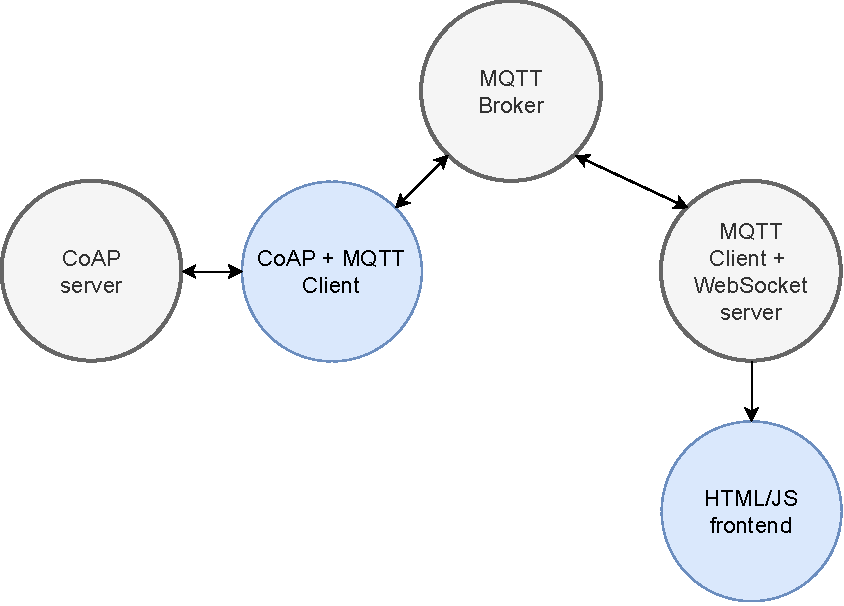
\includegraphics[width=\textwidth]{./doc/system}
		\caption{Overview of the system}
		\label{system-overview}
	\end{center}
\end{figure}

Figure~\ref{system-overview} shows a brief overview of the different components in the system.

\iffalse
With regards to C- and D-level diploma work, it is insufficient to merely perform a practical construction or programming project. A systematic study must also be carried out, e.g. an evaluation and analysis of the design or program. The study should result in objective facts, preferably in the form of tables and diagrams, into which your own conclusions are built in. The study can be a verification of a design that meets the requirement specification, or a comparison of competing alternatives. It is acceptable to allow users to answer a questionnaire or be interviewed. It is also possible to evaluate web-pages and other user interfaces according to usability criteria.

The method section is the point at which your chosen method and intended procedure during the research are discussed. This section shall not be a chronological diary filled with irrelevant details, but should contain information given in such a way that it is understandable for the reader and enables him/her to interpret your results and repeat your work, i.e. in order to check the results. Here, the tools, assumptions, mathematical models, performance measures and assessment criteria are presented. It is also at this point that the means adopted for the evaluation and verification of the computer programs and technical solution proposals are presented. This can include a test plan to check that the structure works and criteria to assess its usefulness. In research reports regarding natural science and technology this chapter is often called “Model”, “System Model” or “Simulation Model”.

Justify your choice of methodology/model. This choice is very important, because it could be the actual key to the result of your research. Comment on the method's possible weaknesses and problems that may arise during actual implementation. Refer to the problem wording in the introduction chapter. It is possible, for example, to write “problem P1 is attempted through the method M1 and problem P2 through…” 

In your report, you should - depending on what the report is about- find information about what you have investigated and how you have gathered and processed data. Possible questionnaires, interview questions and the likes can be presented as appendices. Detailed descriptions concerning experimental formats of possible interest to those wanting to repeat the experiment should also be included in this chapter.
\fi

    \section{Design / Implementation}
\label{ch:impl}
\noindent	

This chapter aims to discuss the implementation details of the system presented in \textit{figure~\ref{system-overview}}.

\subsection{CoAP server}

\begin{figure}[H]
	\begin{center}
		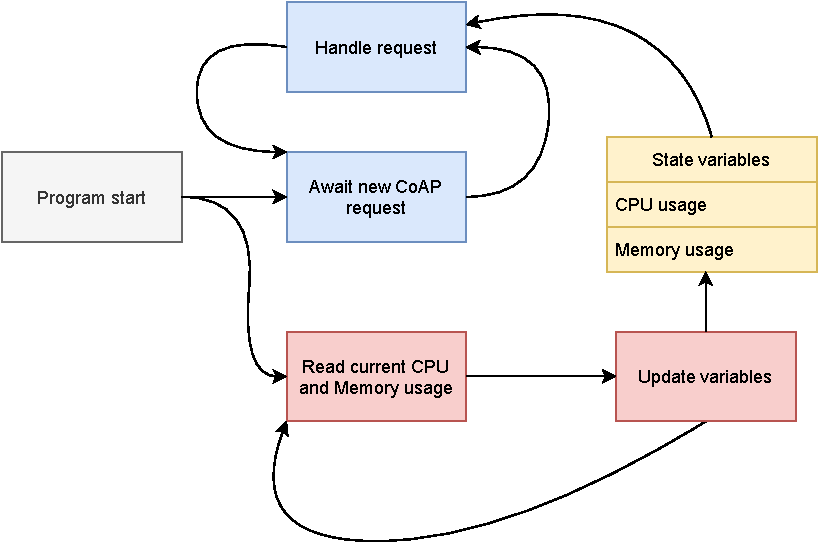
\includegraphics[width=\textwidth]{./doc/coap_flowchart.pdf}
		\caption{Flowchart depicting the duties and the program flow of the CoAP server.}
		\label{coap-figure}
	\end{center}
\end{figure}

\subsection{CoAP + MQTT Client}

\textit{Figure~\ref{coap-figure}} shows the program flow of the CoAP server. The flow is separated into two threads marked as blue and red boxes in figure~\ref{coap-figure}. There is also a yellow box, representing data shared between the threads. This data is locked behind mutex locks so as to not cause any race conditions between the red and blue thread. 

The red thread is responsible for regularly reading the current CPU and memory usage from the system. It then tries to access the shared state variables in order to update them with the new information. Upon successfully updating the variables, the lock is released and the thread sleeps for one second before attempting to read the CPU and memory usage once more.

The blue thread is responsible for performing all server-related duties of the system component. It listens for potential requests to the urls \lstinline{/cpu} and \lstinline{/mem}. Upon recieving a request, it tries to access the corresponding shared state variable, embeds it into a response, and sends the response. It then goes back into listening mode, awaiting the next request.

\subsection{MQTT Broker}

\subsection{MQTT Client + WebSocket server}

\subsection{HTML/JS frontend}

\iffalse
The Design or Implementation chapter often appears in technical reports, but not always in scientific reports. Here, the analysis of the problem is implemented and a technical requirement specification is formulated. At this stage, the most important principles in the suggested alternatives for solution are described and formulated in preparation for evaluation at a later point in the report. The description is sometimes placed before, but generally after the methodology/model chapter, if included at all.

The reader is seldom interested in extremely detailed documentation of computer program code, algorithms, electrical circuit diagrams, user guidance, etc. Such details are placed in the appendices.

As mentioned in the Introduction chapter you have during earlier studies mainly worked with small well defined tasks that have taken minutes or as most hours to solve. In comparison an exam work or a project course can sometimes appear to be an almost overwhelming amount of information because it is so extensive, and this may cause anxiety with regards to where to start. One way to facilitate big projects is to use the top-down-method, i.e. to divide the problem or the structure into smaller problem parts or system parts, and to state specification of  requirements, problem analysis and proposed solution for each part. Eventually small and concrete information will have been identified with similar characteristics to those found in your previous studies.

It is not always practically possible to apply the top-down-method, since the problem may be too complex and initially very difficult to visualise the complete overview. It might prove necessary to alternate between the top-down - and bottom-up-method. The latter means that you start with parts already known to you and from simple problems that have been tackled previously you  make use of that knowledge for aspects that you expect to resolve at a later stage in the project. Gradually increase these parts into the bigger systems and problems and then pursue the direction of project's objective.

The top-down-method has the advantage of giving the report a solid structure, which makes it easier for the reader. The documentation therefore often follows the top-down-method. It is thus possible to divide the structure part into several chapters, and to name them after each problem part and system part, i.e. “Specification of requirements”, “Algorithms”, “User interface”, “Program documentation”, “Prototype” and “Implementation”.
\fi

    \section{Results}
\label{ch:results}
\noindent	
The results chapter is included when you have produced a systematic study, i.e. an evaluation of a program that you have developed, which is required for C - and D-level diploma work. In the results chapter objective results of the empirical study are presented. Keep in mind that possible comments in this chapter should only be used for clarification. Your own views and subjective (personal) comments belong in the chapter conclusion/discussion.

Strive to present the results, for example measurement-, calculations- and/or the simulation result, in a form that is as lucid and easily understandable as possible. The results are preferably presented in diagrams or tables. Accounts of interviews can be summarised, but may include concrete examples supporting your work.

Extensive results, for example complete summaries of survey results, large tables and long mathematical deductions, are placed in the appendices.

    \section{Discussion}
\label{ch:concl}
\noindent	

This project indeed shows that creating a system consisting of several components using different protocols is completely doable. In doing so, the first goal of the project is fulfilled. Likewise, the CoAP client, the MQTT broker and the WebSocket server were all implemented for use within the project, whereas the CoAP server and the MQTT client code were pulled in as external dependencies, meaning that the second goal was also fulfilled. All of these connections could operate with each other as planned, resulting in the fulfillment of the third goal. The fourth goal was also achieved, as could be seen in \textit{chapter~\ref{ch:results}}. The measurements show that the round-trip-time is rather large for a system that is run on a single computer, but one might argue that this could be due to the components being compiled in debug mode. Had more compiler optimizations been turned on, the graph might have ended up looking a little bit differently.

\iffalse
The conclusion/discussion (choose a heading) is a separate chapter in which the results are analysed and critically assessed. At this point your own conclusions, your subjective view, and explanations of the results are presented.

If this chapter is extensive it can be divided up into more chapters or sub-chapters i.e. one analysis or discussion chapter with explanations of and critical assessment of the results, a concluding chapter where the most important results and well supported conclusions are discussed and to sum it up a chapter with suggestions for further research in the same area. In this chapter it is of vital importance that a connection back to the aim of the survey is made and thus the purpose is pointed out in a summary and analysis of the results. 

In this chapter you should also include answers to the following questions: What is the project's news value and its most vital contribution to the research or technology development? Have the project's goals been achieved? Has the task been accomplished? What is the answer to the opening problem formula? Was the result as expected? Are the conclusions general, or do they only apply during certain conditions? Discuss the importance of the choice of method and model for the results. Have new questions arisen due to the result?

The last question invites the possibility to offer proposals to others relevant research, i.e. proposal points for measures and recommendations, points for continued research or development for those wishing to build upon your work. In technical reports on behalf of companies, the recommended solution to a problem is presented at this stage and it is possible to offer a consequence analysis of the solution from both a technical and layman perspective, for example regarding environment, economy and changed work procedures. The chapter then contains recommended measures and proposals for further development or research, and thus to function as a basis for decision-making for the employer or client.
\fi

\subsection{Ethical and Societal Discussion}
\label{ch:concl:ethical}
Something to consider with these protocols is that IoT devices will most likely stay active for several years. All of these years of activity could be summed up into a great amount of energy spent, depending on the situation. It could therefore be of interest to vary the protocol(s) used in order to optimize the energy usage of the system, which in turn could make the entire system "greener". This is of course largely situational depending on the project one wishes to solve, but the proof alone that one can weave different protocols together and still end up with a comprehensible system shows that this is something worth to consider when designing an IoT-centered system. 

\subsection{Future Work}
\label{ch:concl:future-work}
A clear prospect of a future work for this project would be to implement true bi-directional communication for WebSockets. As such, the frontend would be able to request the WebSocket server for the current CPU and memory usage stats, thusly being able to measure the round-trip-time without relying on the WebSocket server to do so. A consequence of this is that the ''true'' round trip time would be measured, instead of just measuring the internal round trip time between the CoAP server and the WebSocket server. As the WebSocket protocol has a somewhat involved decoding step for extracting the payload of the message, it could very well be so that this protocol introduces the largest overhead out of the three protocols used within the project.


    \printbibliography
    \newpage
    \pagestyle{empty}
    
    \pagestyle{fancy}
    \appendix
    \noappendicestocpagenum
    \setcounter{page}{1}

    \counterwithin{figure}{section}
    \counterwithin{table}{section}


	\iffalse
    \begin{appendices}
      \section{Source Code}
\label{appendix:source-code}

\begin{lstlisting}[language=c]
#include <stdio.h>

int main() {
	printf("Hello, World!\n");
}
\end{lstlisting}

    \end{appendices}
	\fi

\end{document}
